\let\negmedspace\undefined
\let\negthickspace\undefined
\documentclass[journal,12pt,onecolumn]{IEEEtran}
\usepackage{cite}
\usepackage{amsmath,amssymb,amsfonts,amsthm}
\usepackage{algorithmic}
\usepackage{graphicx}
\usepackage{textcomp}
\usepackage{xcolor}
\usepackage{txfonts}
\usepackage{listings}
\usepackage{enumitem}
\usepackage{mathtools}
\usepackage{gensymb}
\usepackage{comment}
\usepackage[breaklinks=true]{hyperref}
\usepackage{tkz-euclide} 
\usepackage{gvv}                                        
%\def\inputGnumericTable{}                                 
\usepackage[latin1]{inputenc}     
\usepackage{xparse}
\usepackage{color}                                            
\usepackage{array}                                            
\usepackage{longtable}                                       
\usepackage{calc}                                             
\usepackage{multirow}
\usepackage{multicol}
\usepackage{hhline}                                           
\usepackage{ifthen}                                           
\usepackage{lscape}
\usepackage{tabularx}
\usepackage{array}
\usepackage{float}
\newtheorem{theorem}{Theorem}[section]
\newtheorem{problem}{Problem}
\newtheorem{proposition}{Proposition}[section]
\newtheorem{lemma}{Lemma}[section]
\newtheorem{corollary}[theorem]{Corollary}
\newtheorem{example}{Example}[section]
\newtheorem{definition}[problem]{Definition}
\newcommand{\BEQA}{\begin{eqnarray}}
\newcommand{\EEQA}{\end{eqnarray}}
\newcommand{\define}{\stackrel{\triangle}{=}}
\theoremstyle{remark}
\newtheorem{rem}{Remark}
% Marks the beginning of the document
\begin{document}
\title{2.2.14}
\author{AI25btech11022 - Narshitha}
\maketitle
\renewcommand{\thefigure}{\theenumi}
\renewcommand{\thetable}{\theenumi}
\textbf{Question}:\\
The angle between the line \\
\begin{align}
\vec{r}=\brak{5\hat{i}-\hat{j}-4\hat{k}}+\lambda\brak{2\hat{i}-\hat{j}+\hat{k}}
\end{align}
and the plane 
\begin{align}
   \vec{r}.\brak{3\hat{i}-4\hat{j}-\hat{k}}+5=0
\end{align}
is\\
\textbf{Solution}:
The given line can be expressed in the form as \\
\begin{align}
    \vec{r}=\myvec{5\\-1\\-4}+\lambda\myvec{2\\-1\\1}
\end{align}
Hence the vector direction of this line is
\begin{align}
    \myvec{2\\-1\\1}
\end{align}
the normal vector of the given plane is
\begin{align}
    \myvec{3\\-4\\-1}
\end{align}
by the formula
\begin{align}
    \cos\theta=\frac{\vec{a}^T\vec{b}}{\|\vec{a}\|\|\vec{b}\|}
\end{align}
Thus the cosine of the angle between the two is
\begin{align}
\frac{3\sqrt{3}}{2\sqrt{13}}
\end{align}
which is sine of the angle between the plane and the line.\\
$\therefore$ The angle between the line and plane is $\sin^{-1}\frac{3\sqrt{3}}{2\sqrt{13}}$
\begin{figure}
    \centering
    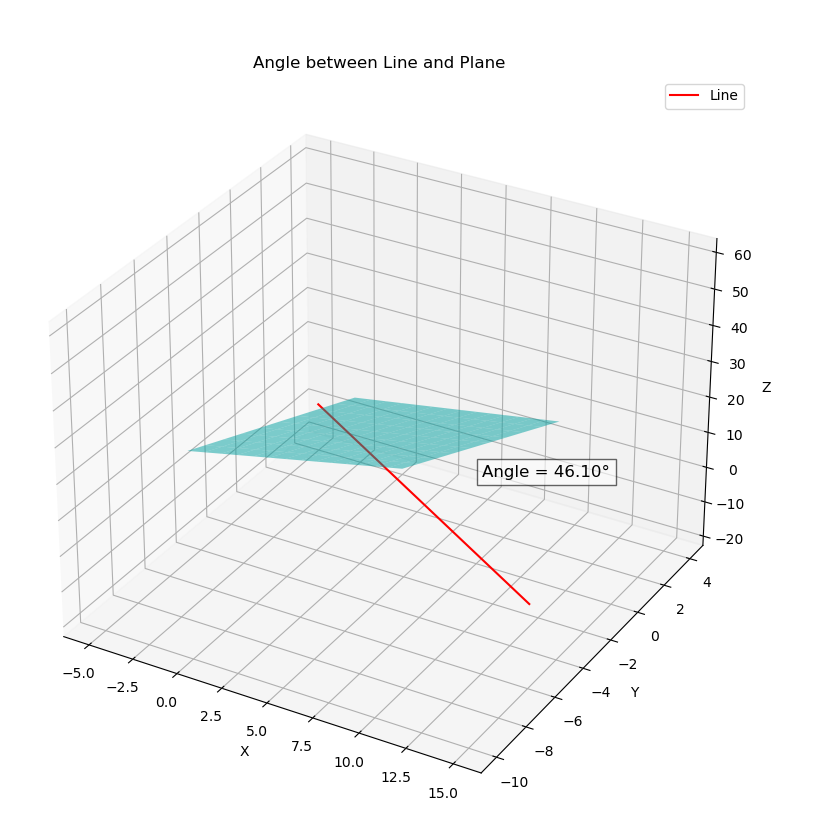
\includegraphics[width=0.5\linewidth]{figs/fig1.png}
    \caption{Caption}
    \label{fig:placeholder}
\end{figure}
\end{document}
